\subsection{Thread Scheduling}\label{subsec:Thread_Scheduling}
\begin{blackbox}
  \textbf{On operating systems that support them, \nameref{def:Kernel_Thread}s, not \nameref{def:Process}es are scheduled by the operating system.}
  However, the terms ``process scheduling'' and ``thread scheduling'' are often used interchangeably.
  Process scheduling is used when discussing general scheduling concepts and thread scheduling to refer to thread-specific ideas.
\end{blackbox}

\subsubsection{User- vs. Kernel-Level Thread Scheduling}\label{subsubsec:User_vs_Kernel_Thread_Scheduling}
On systems implementing the \nameref{subsubsec:Many_To_One_Model} (\Cref{subsubsec:Many_To_One_Model}) and \nameref{subsubsec:Many_To_Many_Model} (\Cref{subsubsec:Many_To_Many_Model}), the thread library schedules user-level threads to run on an available LWP.\@

\begin{definition}[Process-Contention Scope]\label{def:Process_Contention_Scope}
  \emph{Process-Contention Scope} is where each of the \nameref{def:Thread}s \textbf{WITHIN A SINGLE \nameref{def:Process}} compete with each other for execution.
\end{definition}

In \nameref{def:Process_Contention_Scope}, the \nameref{def:Thread_Library} schedules the \nameref{def:User_Thread}s onto available \nameref{def:Lightweight_Process}es, or directly onto \nameref{def:Kernel_Thread}s.
However, this does not mean that the \nameref{def:User_Thread} are being scheduled for execution.
For that to happen, the \nameref{def:Kernel} must be involved.

To decide what \nameref{def:Thread}s can execute on the CPU, we broaden our view of contention to \nameref{def:System_Contention_Scope}.

\begin{definition}[System-Contention Scope]\label{def:System_Contention_Scope}
  \emph{System-Contention Scope} is where \textbf{ALL} of the \nameref{def:Thread}s on the system, from all \nameref{def:Process}es compete with each other for execution.
\end{definition}

If a \nameref{def:Kernel} uses the \nameref{subsubsec:One_To_One_Model}, then \textbf{ALL} threads are scheduled using \nameref{def:System_Contention_Scope}.

\subsubsection{Multiprocessor Scheduling}\label{subsubsec:Multiprocessor_Scheduling}
If multiple processors are available for use in a system, then \nameref{def:Load_Sharing} is possible.

\begin{definition}[Load Sharing]\label{def:Load_Sharing}
  \emph{Load sharing} involves splitting the load of running \nameref{def:Process}es and their \nameref{def:Thread}s between multiple processors.
  This does not limit the possibility of multithreading, rather it complements it.
\end{definition}

In this course, we consider each processor to be equivalent, or homogenous.
This means that each one will have the same basic set of functionality and can reach all resources present in the system.
This does not mean that all processors can reach all the resources with the same cost/delay.
There may be an I/O device attached to the private bus of a core, or there may be \nameref{def:Non_Uniform_Memory_Access}.

\paragraph{Approaches to Multiprocessor Scheduling}\label{par:Multiprocessor_Scheuling_Approaches}
There are 2 main approaches to multiprocessor scheduling, without taking the idea of non-uniform resource availability.
\begin{enumerate}[noitemsep]
\item \nameref{def:Asymmetric_Multiprocessor_System}
\item \nameref{def:Symmetric_Multiprocessor_System}
\end{enumerate}

In an \nameref{def:Asymmetric_Multiprocessor_System}, one of the processors acts as the master server.
It runs the scheduler, allocating jobs to each of the slave worker processors.
This reduces the need for data sharing, making coding and debugging such a thing much easier.

The other approach, \nameref{def:Symmetric_Multiprocessor_System}, allows each processor to schedule itself.
Tasks to execute may be in 2 types of queues:
\begin{enumerate}[noitemsep]
\item A common queue for all processors.
\item A private queue, one for each processor.
\end{enumerate}

Each processor must select a job from the ready queue and execute it.
We must ensure that no two processors schedule and execute the same task at the same time, and that processes are not lost from the queue.

\begin{blackbox}
  Throughout this section, and most of this document, we discuss \nameref{def:Symmetric_Multiprocessor_System} (SMP) systems.
  These are more commonly in use in the desktop space and are more interesting to discuss.
\end{blackbox}

\subsubsection{Processor Affinity}\label{subsubsec:Processor_Affinity}
\nameref{def:Process}es/\nameref{def:Thread}s can migrate between processors, no matter the type of multiprocessor system used.
However, if such a migration happens, the processor's cache must be invalidated from the origin and the destination cache must be populated.
This is a very high cost to system productivity, so we attempt to keep a \nameref{def:Process}/\nameref{def:Thread} running on the same processor for as long as possible, this is known as \nameref{def:Processor_Affinity}.

\begin{definition}[Processor Affinity]\label{def:Processor_Affinity}
  \emph{Processor affinity} is the idea of keeping one \nameref{def:Process}/\nameref{def:Thread} running on the \textbf{same} processor for as long as possible.
  This prevents relatively costly process migrations from becoming common.

  There are 2 kinds of processor affinity:
  \begin{enumerate}[noitemsep]
  \item \nameref{def:Soft_Affinity}
  \item \nameref{def:Hard_Affinity}
  \end{enumerate}
\end{definition}

\begin{definition}[Soft Affinity]\label{def:Soft_Affinity}
  \emph{Soft affinity} is where \nameref{def:Processor_Affinity} is used, but no guarantees about the migration of a \nameref{def:Process} can be made.
  The \nameref{def:Operating_System} will attempt to keep a process running on the same processor for as long as possible, but the process can still migrate between processors.
\end{definition}

\begin{definition}[Hard Affinity]\label{def:Hard_Affinity}
  \emph{Hard affinity} is where once a \nameref{def:Process}/\nameref{def:Thread} is assigned to a set of processors, it will \textbf{ONLY EXECUTE ON THOSE}.
\end{definition}

The organization of \nameref{def:Memory} in a system will affect the performance of the \nameref{def:Processor_Affinity} choices made.
In a \nameref{def:Non_Uniform_Memory_Access} system, not all memory is \textbf{DIRECTLY} available to every processor.
In this type of system, a \nameref{def:Process}'s affinity should be set according to the memory location it inhabits.
Otherwise, there will be long delays during memory acccesses.
This is illustrated in \Cref{fig:NUMA_Multiprocessor_Scheduling}.

\begin{figure}[h!tbp]
  \centering
  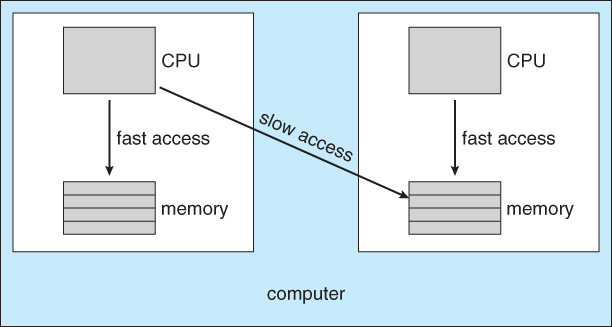
\includegraphics[scale=1.00]{./Drawings/EDAF35-Operating_Systems/NUMA_Multiprocessor_Scheduling.jpg}
  \caption{\nameref*{def:Non_Uniform_Memory_Access}, \nameref*{def:Processor_Affinity}, and \nameref*{rmk:CPU_Scheduler} Choices}
  \label{fig:NUMA_Multiprocessor_Scheduling}
\end{figure}


%%% Local Variables:
%%% mode: latex
%%% TeX-master: "../../EDAF35-Operating_Systems-Reference_Sheet"
%%% End:
